\documentclass[14pt]{beamer}

% Presento style file
\usepackage{config/presento}

% custom command and packages
% custom packages
\usepackage{textpos}
\setlength{\TPHorizModule}{1cm}
\setlength{\TPVertModule}{1cm}

\newcommand\crule[1][black]{\textcolor{#1}{\rule{2cm}{2cm}}}



% Information
\title{Segundo Seminario}
\subtitle{algo con machine learning}
\author{Bruno S\'anchez \& \\
Mariano Dom\'{\i}guez}
%\titlegraphic{
\includegraphics[scale=0.8]{./images/vitraux_h90.png}}
\institute{IATE - FaMAFyC\\

\includegraphics[scale=0.8]{./images/vitraux_h90.png}}
\date{\today}

\begin{document}

% Title page
\begin{frame}[plain]
\maketitle
\end{frame}

% sections in the presentation
\begin{frame}{Resumen}
 \begin{fullpageitemize}
  \item \largetext{Motivaciones}
  \item \largetext{Las diferencias de im\'agenes}
  \item \largetext{Pipelines con Corral}
  \item \largetext{Simulaciones de im\'agenes}
  \item \largetext{Datos reales}
  \item \largetext{Machine Learning}
 \end{fullpageitemize}
\end{frame}

\begin{frame}
\frametitle{Contenidos}
\tableofcontents%[sectionstyle=show/hide, 
    %sectionstyle=show/shaded]
\end{frame}


\section{Motivaciones}

\begin{frame}{Las variaciones en el cielo}
    \begin{figure}
        \centering
        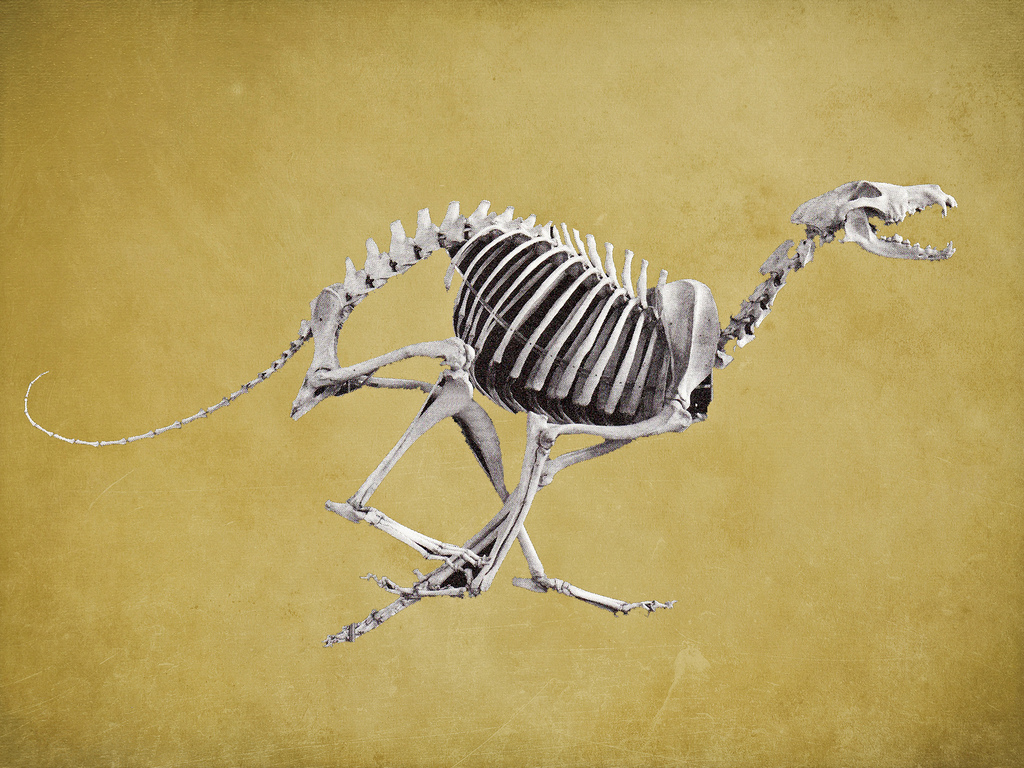
\includegraphics[width=0.8\textwidth]{./images/skeleton.jpg}
        \caption{Diagrama de variabilidad}
        \label{fig:diag_vacio}
    \end{figure}
\end{frame}

\section{Las diferencias de Im\'agenes}
\section{Pipelines de datos}
\section{Simulaciones de Im\'agenes}
\section{Datos Reales}
\section{Machine Learning}




\begin{frame}{Open Source Fonts}
 \begin{fullpageitemize}
  \item {\montserratfont This is Montserrat}
  \item {\notosansfont This is Noto Sans}
  \item {\latolightfont This is Lato (light)}
  \item {\inconsolatafont This is inconsolata}
  \item \textsc{This is Alegreya Sans small caps}
 \end{fullpageitemize}
\end{frame}

\begin{frame}{Color Palette}
 \begin{center}
  \crule[colordgray] \crule[colorhgray] \crule[colorblue] \crule[colorgreen] \crule[colororange]
 \end{center}
\end{frame}

\framecard[colorgreen]{{\color{white}\hugetext{BIG BOLD TEXT}}}

\framepic[0.8]{images/skeleton}{
 \begin{textblock}{7}(7,2.5)
    {\color{colorblue}\hugetext{\textbf{RUN!}}}
 \end{textblock}
}
\end{document}